\section{Pulsar Wind Nebula}
\label{sec:PWN}

Unlike supernova remnants,
the pulsar wind nebulae are continuously renewed in energy
and are visible for much longer than supernova remnants.

Energy from the pulsar rotation is dissipated into the pulsar wind.
This dissipated spin down energy is given as
\begin{equation}
\dot{E}=I \Omega \dot{\Omega}
\end{equation}
where $I$ is the moment of inertia of the spinning neutron star and $\Omega$
is the angular frequency of the rotation.

The angular frequency and change in the angular frequency are
assumed to be related to each other as
\begin{equation}\label{eq:angFreq}\dot{\Omega} \propto \Omega^n\end{equation}
where $n$ is the braking index.
Using this relationship, one can solve for the age of the pulsar.

\begin{figure}[t!!]
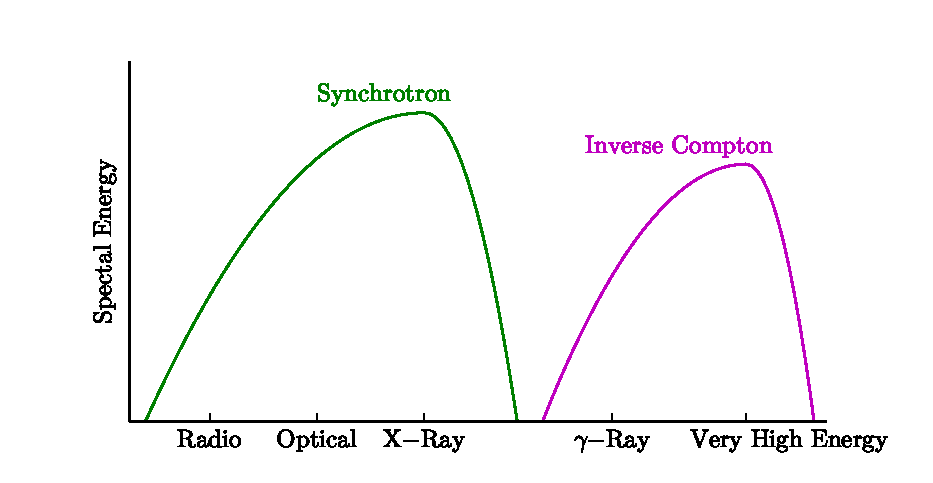
\includegraphics[width=.95\textwidth]{chapters/pulsarAnatomy/figures/spec.eps}
\caption[Typical pulsar wind nebula energy spectrum]{
\label{spec} Typical pulsar wind nebula energy spectrum.
Inspired by Figure 1.1 of \cite{vanEttenPhd2012}.}
\end{figure}

Interaction of this outflow with surrounding medium creates emission.
Particles interact with magnetic fields and photons to produce
synchrotron (very relativistic and ultra-relativistic electrons
gyrating in a magnetic field)
and inverse Compton (scattering of low energy photons
to high energy by ultra-relativistic electrons) emission. For
younger pulsars, this medium includes the cold supernova ejecta
beyond the termination shock.
Termination shock forms where the ram pressure of the wind 
balances the pressure of the surrounding medium.  
Figure~\ref{spec} shows a typical energy spectrum of a pulsar
wind nebula.


Of particular interests to polarization and geometric modeling
(the main theme of this thesis)
is the X-ray torus of pulsar wind nebulas which is further discussed
in Section \ref{subsec:ToriModeling}.
For more detailed overview of pulsar wind nebula see \cite{vanEttenPhd2012}
and
\cite{gaensler2006evolution}.
